\section{Effective Number of Neutrinos  in the Instantaneous  Freeze-out Model}\label{ch:model_ind}

The effective number of neutrinos, $N^{\text{eff}}_\nu$, quantifies the amount of radiation energy density, $\rho_r$, in the Universe prior to photon freeze-out and after $e^\pm$ annihilation.  $N^{\text{eff}}_\nu$ is a key comological observable that can be  measured by fitting to the distribution of CMB temperature fluctuations. The  Planck~\cite{Planck}  analysis gives $N^{\text{eff}}_{\nu}=3.36\pm 0.34$ (CMB only) and $N^{\text{eff}}_{\nu}=3.62\pm 0.25$ (CMB+$H_0$) ($68\%$ confidence levels), indicating a possible tension in the current understanding of $N^{\text{eff}}_\nu$.   This section, as well as in Section \ref{ch:param_studies}, works towards a detailed understanding of $N^{\text{eff}}_{\nu}$ with an eye towards this tension.

Mathematically, $N^{\text{eff}}_\nu$ is defined by the relation
\begin{align}\label{eq:N_eff_def}
\rho_r=\left(1+(7/8)R_\nu^{4}N^{\text{eff}}_\nu\right)\rho_\gamma\,,
\end{align}
where $\rho_r$ is the radiation component of the Universe  energy density, $\rho_\gamma$ is the photon energy density and  $R_\nu\equiv T_\nu/T_\gamma=({4}/{11})^{1/3}$ is the photon to neutrino temperature ratio in the limit where  the annihilating $e^\pm$ pairs do not transfer any entropy  to  Standard Model (SM) left-handed neutrinos, i.e., under the assumption that neutrinos have completely frozen out at the time of $e^\pm$ annihilation.  The factor 7/8 is the ratio of Fermi to Bose reference normalization in $\rho$ and the neutrino to photon temperature ratio $R_\nu$ is the result of the transfer of $e^\pm$ entropy into photons after  neutrino freeze-out.  

The definition \ref{eq:N_eff_def} is constructed such that if photons and SM left-handed neutrinos are the only significant massless particle species in the Universe between the freeze-out of left-handed neutrinos at  $T_\gamma=\mathcal{O}(1)$ MeV and photon freeze-out at $T_\gamma=0.25$ eV, and assuming zero reheating of neutrinos, then $N^{\text{eff}}_{\nu}=3$, corresponding to the number of SM neutrino flavors.  Detailed numerical study of the neutrino freeze-out process within the SM gives $N^{\text{eff}}_{\nu}=3.046$~\cite{Mangano2005}, a value close to the number of flavors, indicating only a small amount of neutrino reheating.  
 We emphasize that $N^{\text{eff}}_\nu$ is named after neutrinos as they are the only significant contributor in SM cosmology. However,   $N^{\text{eff}}_\nu$ could be impacted by non SM particles.

In Sections \ref{EVEq} - \ref{Tnugam} we study how $N^{\text{eff}}_{\nu}$ is impacted by non-SM neutrino dynamics by characterizing its dependence on the neutrino freeze-out temperature within an instantaneous freeze-out model.  This model, based on the work in \cite{Birrell2013,Birrell:2013_2}, allows us study $N^{\text{eff}}_{\nu}$ without  requiring a detailed description of the underlying  non-SM interactions; the latter will be considered later in Section \ref{ch:param_studies}.   In addition, in Section  \ref{sec:Neff_QGP}, we explore the possibility of non-SM neutrino contributions to $N^{\text{eff}}_\nu$; this latter section is based on \cite{Birrell:2014cja}.






\subsection{Chemical and Kinetic Equilibrium }\label{EVEq}

As the Universe expands and cools, the various components of the Universe transition  from equilibrium to non-interacting. This process is governed by two key temperatures: 1) The chemical freeze-out temperature, $T_{ch}$, above which the particles are kept in chemical  equilibrium by number changing interactions. 2) The  kinetic freeze-out temperature, above which the particles are kept in thermal equilibrium, i.e., equilibrium momentum distribution.  In reality, these are not sharp transitions, but we approximate them as such in this section.  The insights gained here will be important when studying the more detailed model of neutrino freeze-out in later sections.



At sufficiently high temperatures, such as existed in the early Universe, both particle creation and annihilation (i.e. chemical) processes and momentum exchanging (i.e. kinetic) scattering processes can occur sufficiently rapidly to establish complete thermal equilibrium of a given particle species. The  distribution function $f_{ch}^\pm$ of  fermions (+) and bosons (-) in both chemical and kinetic equilibrium is found by maximizing entropy subject to energy being conserved
\begin{equation}\label{ch_eq}
f_{ch}^\pm=\frac{1}{\exp(E/T)\pm 1}, \hspace{2mm} T>T_{ch}
\end{equation}
where $E$ is the particle energy, $T$ the temperature, and $T_{ch}$ the chemical freeze-out temperature. 



As temperature decreases, there will be a period where the temperature is greater than the kinetic freeze-out temperature, $T_k$, but below chemical freeze-out. During this period, momentum exchanging processes continue to maintain an equilibrium distribution of energy among the available particles, which we call kinetic equilibrium, but particle number changing processes no longer occur rapidly enough to keep the equilibrium particle number yield, i.e. for $T<T_{ch}$ the particle number changing processes have `frozen-out'. In this condition the momentum distribution, which is in kinetic equilibrium but chemical non-equilibrium, is obtained by maximizing  entropy subject to  particle number and energy constraints and thus two parameters appear
\begin{equation}\label{k_eq}
f_{k}^\pm=\frac{1}{\Upsilon^{-1} \exp(E/T)\pm 1},\hspace{2mm} T_k<T\leq T_{ch}.
\end{equation}
The need to preserve the total particle number within the distribution introduces an additional parameter $\Upsilon$ called fugacity. 



The fugacity, $\Upsilon(t)\equiv e^{\sigma(t)}$, controls the occupancy of phase space and is necessary once $T(t)<T_{ch}$ in order to conserve particle number.  A fugacity different from $1$ implies an over-abundance ($\Upsilon>1$) or under-abundance ($\Upsilon<1$) of particles compared to chemical equilibrium and in either of these  situations one speaks of chemical non-equilibrium. 

The effect of $\sigma$ is similar after that of chemical potential $\mu$, except that $\sigma$ is equal for particles and antiparticles, and not opposite. This means $\sigma>0$ ($\Upsilon>1$) increases the density of both particles and antiparticles, rather than increasing one and decreasing the other as is common when the chemical potential is associated with conserved quantum numbers.  Similarly, $\sigma<0$ $(\Upsilon<1)$ decreases both. The fact that $\sigma$ is not opposite for particles and antiparticles reflects the fact that both  the number of particles and the number of antiparticles are conserved after chemical freeze-out, and not just their difference.  Ignoring the small particle antiparticle asymmetry their equality reflects the fact that any process that modifies  the distribution would affect both particle and antiparticle distributions in the same fashion.   Such an asymmetry would be incorporated by replacing $\Upsilon\rightarrow \Upsilon e^{\pm\mu/T}$ where $\mu$ is the chemical potential, but we ignore it in this work as the matter antimatter asymmetry is on the order of $1$ part in $10^9$.

 We also emphasize that the fugacity is time dependent and not just an initial condition.  At high temperatures $\Upsilon=1$ and we will find that $\Upsilon<1$ emerges dynamically as a result of the freeze-out process. The importance of fugacity was first introduced in \cite{PhysRevLett.48.1066} in the context of quark-gluon plasma.  Its presence in cosmology was noted in  \cite{Bernstein:1985,Dolgov:1993} but its importance has been largely forgotten and the consequences unexplored in the literature.  





\subsubsection{Dynamics and Conservation Laws}
In a flat FRW universe, the spacial components of the divergence of the stress energy tensor automatically vanish, leaving the single condition
\begin{equation}\label{stress_energy_eq}
\nabla_\mu \mathcal{T}^{\mu 0}=\dot{\rho}+3\left(\rho+P\right)\frac{\dot{a}}{a}=0.
\end{equation}
If the set of particles can be portioned into subsets such that there is no interaction between the different subsets then this condition applies independently to each and leads to an independent temperature for each such subset.  We will focus on a single such group and use \req{stress_energy_eq}  to derive an equivalent condition involving entropy and particle number, which illustrate how the entropy of the universe evolves in time. 

Consider a  collection of particles in kinetic equilibrium at a common temperature $T$, with distinct fugacities $\Upsilon_i$, and  which satisfy \req{stress_energy_eq}.   For the following derivation, it is useful to define $\mu_i=\sigma_i T$.  This gives the expressions a familiar thermodynamic form with $\mu$ playing the role of chemical potential and helps with the calculations, but should not be confused with a chemical potential as discussed above.  The expressions for the  energy density, pressure, number density, and entropy density of a particle of mass $m$ with momentum distribution $f$ are
\begin{align}\label{moments}
\rho=&\frac{g_p}{(2\pi)^3}\int f(t,p)Ed^3p\,,\\
P=&\frac{g_p}{(2\pi)^3}\int f(t,p)\frac{p^2}{3E}d^3p\,,\\
n=&\frac{g_p}{(2\pi)^3}\int f(t,p) d^3p, \hspace{2mm} E=\sqrt{m^2+p^2}\,,\\
s=&-\frac{g_p}{(2\pi)^3}\int (f\ln(f)\pm(1\mp f)\ln(1\mp f)) d^3p\,,
\end{align}
where $g_p$ is the degeneracy of the particle.

Integration by parts establishes the following identities when $f=f_i$ is the kinetic equilibrium distribution \req{k_eq} for the $i$'th component:
\begin{equation}\label{identities}
s_i=\frac{\partial P_i}{\partial T}=(P_i+\rho_i-\mu_i n_i)/T, \hspace{3mm} n_i=\frac{\partial P_i}{\partial \mu_i}.
\end{equation}
Combining \req{stress_energy_eq} with the identities in \req{identities} we can obtain the rate of change of the total comoving entropy as follows.  Letting $s=\sum_i s_i$ be the total entropy density, first compute
\begin{align}\frac{1}{a^3}\frac{d}{dt}(a^3sT)&=\frac{1}{a^{3}}\frac{d}{dt}(a^3(P+\rho-\sum_i \mu_i n_i))\\
&=\dot{P}+\dot{\rho}-\sum_i \left(\dot{\mu_i}n_i+\mu_i\dot{n_i}\right)+3\left(P+\rho-\sum_i \mu_i n_i\right)\dot{a}/a\notag\\
&=\frac{\partial P}{\partial T} \dot{T}+\sum_i\frac{\partial P_i}{\partial \mu_i} \dot{\mu_i}-\sum_i \left(\dot{\mu_i}n_i+\mu_i\dot{n_i}+3\mu_i n_i \dot{a}/a\right)+\nabla_\mu \mathcal{T}^{\mu 0}\notag\\
&=s\dot{T}-\sum_i \left(\mu_i\dot{n_i}+3\mu_i n_i \dot{a}/a\right)\notag\\
&=s\dot{T}- a^{-3}\sum_i\mu_i\frac{d}{dt}(a^3n_i)\,.\notag
\end{align}
Therefore we find
\begin{align}\label{S_n_eq}
\frac{d}{dt}(a^3s)=&\frac{1}{T}\frac{d}{dt}(a^3sT)-a^3s\frac{\dot T}{T}=-\sum_i\sigma_i\frac{d}{dt}(a^3n_i).
\end{align}
From this we can conclude that comoving entropy in conserved as long as every particles satisfies one of the following  conditions: 1) The particle is  in chemical equilibrium, i.e. $\sigma_i= 0$. 2) The particle has frozen out chemically and thus has conserved comoving particle number, i.e., $\frac{d}{dt}(a^3n_i)$.  Therefore, under the instantaneous freeze-out assumption, we can conclude  conservation of comoving entropy. 


These observations provide an alternative characterization of the dynamics of a FRW universe that is composed of entirely of particles in chemical or kinetic equilibrium.  The dynamical quantities are the scale factor $a(t)$, the common temperature $T(t)$, and the fugacities of each particle species $\Upsilon_i(t)$ that is not in chemical equilibrium.  The dynamics are given by the Einstein equation, conservation of the total comoving entropy of all particle species, and conservation of comoving particle number for each species not in chemical equilibrium (otherwise $\Upsilon_i=1$ is constant)
\begin{equation}\label{eq_dynamics}
H^2=\frac{\rho_{tot}}{3M_p^2}, \hspace{2mm} \frac{d}{dt}(a^3s)=0,\hspace{2mm} \frac{d}{dt}(a^3n_i)=0 \text{ when } \Upsilon_i\neq 1.
\end{equation}
We emphasize here that $\rho_{tot}$ is the total energy density of the Universe, which may be composed of contributions from multiple particle groupings with no cross goup interactions. In such case, each grouping has its own temperature and   independently conserves its comoving entropy. 



%%%%%%%%%%%%%%%%%%%%%%%%%%%%%%%%%%%%%%%%%%%%%%%
\subsection{Einstein-Vlasov Equation in FRW Spacetime}\label{sec:free_stream_sol}
Once the temperature drops below the kinetic freeze-out temperature $T_k$ of a particular component of the Universe, we reach  the free streaming period where  particle scattering processes have completely frozen out. The   dynamics are therefore determined by the free-streaming Boltzmann-Einstein equation (\req{boltzmann_einstein} with $C[f]=0$), known as the Einstein-Vlasov equation, in a spatially flat FRW universe.  Due to the assumed homogeneity and isotropy, the particle distribution function depends on $t$ and $p^0=E$ only and so the Einstein-Vlasov equation becomes
\begin{equation}\label{VEeqFLR}
E\partial_tf+(m^2-E^2)\frac{\partial_ta}{a}\partial_{E}f=0.
\end{equation}
The general solution to \req{VEeqFLR} can be found in, e.g., ~\cite{bruhat,Wong}:
\begin{equation}\label{general_sol}
f(t,E)=K(x),\hspace{3mm} x\equiv\frac{a(t)^2}{D^2}(E^2-m^2),
\end{equation}
where $K$ is an arbitrary smooth function and $D$ is an arbitrary constant with units of mass.  To continue the evolution beyond thermal freeze-out  we choose $K$ to match the kinetic equilibrium distribution \req{k_eq} at the freeze-out time $t_k$. For neutrinos, this is accomplished by setting
\begin{equation}\label{K_func}
K(x)=\frac{1}{\Upsilon_\nu^{-1}e^{\sqrt{x+m^2/T_k^2}}+ 1}
\end{equation}
and $D=T_k a(t_k)$. The Fermi-Dirac-Einstein-Vlasov (FDEV) distribution function for neutrinos after freeze-out is then
\begin{equation}\label{neutrino_dist}
f(t,E)=\frac{1}{\Upsilon_\nu^{-1}e^{\sqrt{(E^2-m^2)/T_\nu^2+m_\nu^2 /T_k^2}}+ 1}
\end{equation}
where 
\begin{equation}\label{Tneutrino_dist}
T_\nu(t)=\frac{T_ka(t_k)}{a(t)}.  
\end{equation}
\req{neutrino_dist} describes a gas of neutrinos that is free streaming in an expanding universe ever since the freeze-out temperature $T_\nu(t_k)=T_k$. We will call $T_\nu$ in \req{Tneutrino_dist} the neutrino background temperature, even though  the distribution of free streaming particles has a thermal shape only for $m=0$ and hence $T_{\nu}$ will differ from the temperature of the photon background.   

The energy, pressure, number density, and entropy density of the free-streaming distribution can be computed using \eqref{Tmndef}, \eqref{nmdef}, and \eqref{smdef},
\begin{align}
\rho&=\frac{g_\nu}{2\pi^2}\!\int_0^\infty\!\!\!\frac{\left(m_\nu^2+p^2\right)^{1/2}p^2dp }{\Upsilon_\nu^{-1}e^{\sqrt{p^2/T_\nu^2+m_\nu^2/T_k^2}}+ 1}\,,\label{neutrino_rho}\\[0.2cm]
P&=\frac{g_\nu}{6\pi^2}\!\int_0^\infty\!\!\!\frac{\left(m_\nu^2+p^2\right)^{-1/2}p^4dp }{\Upsilon_\nu^{-1} e^{\sqrt{p^2/T_\nu^2+m_\nu^2/T_k^2}}+ 1}\,,\label{neutrino_P}\\[0.2cm]
n&=\frac{g_\nu}{2\pi^2}\!\int_0^\infty\!\!\!\frac{p^2dp }{\Upsilon_\nu^{-1}e^{\sqrt{p^2/T_\nu^2+m_\nu^2/T_k^2}}+ 1}\,,\label{num_density}\\
s&=-\frac{g_\nu}{2\pi^2}\!\int_0^\infty\!\!\!H(z^2/T_\nu^2)z^2dz\,,\,\,\,H\equiv K\ln K +(1-K)\ln(1-K)\,,\label{entropy_integrand}
\end{align}
where $g_\nu$ is the neutrino degeneracy (not to be confused with the metric factor $\sqrt{-g}=a^3)$.
Comparing these to the corresponding quantities in Minkowski space, we see that they differ by the replacement $m\rightarrow m T_\nu(t)/T_k$ in the exponential factor  {\em only}.  Changing variables to $u=p/T_\nu$, one sees that both $n$ and $s$ are proportional to $T_\nu^3$.  The neutrino free-straming temperature, $T_\nu$, is inversely proportional to $a$, hence we see that
\begin{equation}\label{const_entropy}
a^3n=\text{constant}\text{ and } a^3s=\text{constant}.
\end{equation}
This proves that the particle number and entropy in a comoving volume are conserved, irrespective of the  form of $K$ that defines the shape of the momentum distribution at freeze-out. 

%%%%%%%%%%%%%%%%%%%%%%%%%%%%%%%%%%%%%%%%%%%%%%%%%%%%%%%%%%%%%%%%%%%%%%%%%%%%%%%%%%%%%%%%%%
\subsection{Neutrino Fugacity and Photon to Neutrino Temperature Ratio}\label{Tnugam}
The instantaneous freeze-out assumption allows us to use conservation laws in \req{eq_dynamics} to characterize the neutrino fugacity and temperature in terms of the freeze-out temperature $T_k$.  We first outline the physics of the situation qualitatively. For $T_k<T<T_{ch}$, the evolution of the temperature of the common $e^\pm,\gamma,\nu$ plasma and the neutrino fugacity are determined by conservation of comoving neutrino number (since $T<T_{ch}$) and conservation of entropy.    As shown in Section \ref{sec:free_stream_sol}, after thermal freeze-out the neutrinos begin to free-stream and therefore $\Upsilon_\nu$ is constant, the neutrino temperature evolves as $1/a$, and the comoving neutrino entropy and neutrino number are exactly conserved.  The photon temperature then evolves to conserve the comoving entropy in photons, electrons, and positrons.  As annihilation occurs, entropy from $e^+e^-$ is fed into photons, leading to reheating.  We now make this analysis quantitative in order to derive a relation between the reheating temperature ratio and neutrino fugacity.

Assuming $T_{ch}\gg m_e$, the entropy in a given comoving volume, $V(t_{ch})$, is the sum of relativistic neutrinos (with $\Upsilon_\nu=1$), electrons, positrons, and photons
\begin{equation}
S(T_{ch})=\left(\frac{7}{8}g_\nu+\frac{7}{8}g_{e^\pm} +g_\gamma \right)\frac{2\pi^2}{45} T_{ch}^3V(t_{ch})\,,
\end{equation}
where $T_1$ is the common neutrino, $e^+e^-$, and $\gamma$ temperature. The number of neutrinos and anti-neutrinos in this same volume is
\begin{equation}
\mathcal{N}_\nu(T_{ch})=\frac{3g_\nu}{4\pi^2}\zeta(3)T_1^3V(t_{ch})\,.
\end{equation}
The particle-antiparticle, flavor, and spin-helicity statistical factors are $g_\nu=6$, $g_{e^\pm}=4$, $g_\gamma=2$.

Distinct chemical and thermal freeze-out temperatures lead to a non-equilibrium modification of the neutrino distribution in the form of a fugacity factor $\Upsilon_\nu$ when $T_k<T<T_{ch}$.  This leads to the following expressions for neutrino entropy and number at $T=T_k$ in the comoving volume
\begin{align}
S(T_k)=&\left(\frac{2\pi^2}{45}g_\gamma T_k^3+S_{e^\pm}(T_k)+S_{\nu}(T_k)\right)V(t_k)\,,\\
\mathcal{N}_{\nu}(T_k)=&\frac{g_\nu}{2\pi^2}\int_0^\infty \frac{u^2 du}{\Upsilon_\nu^{-1}(T_k)e^u+1}T_k^3V(t_k)\,.\notag
\end{align}

After neutrino freeze-out and when $T_{\gamma}\ll m_e$, the entropy in neutrinos is conserved independently of the other particle species and the $e^+e^-$ entropy is nearly all transferred to photons:
\begin{equation}
S_{\gamma}(T_\gamma)=\frac{2 \pi^2}{45}g_\gamma T_{\gamma}^3 V(t).
\end{equation}
 Note that we must now distinguish between the neutrino and photon temperatures.

 %%%%%%%%%%%%%%%%%%%%%%%%%%%%%%%%%%%%%%%
\begin{figure}\label{fig:Tk_dependence}
\begin{minipage}{\linewidth}
\makebox[0.47\linewidth]%
{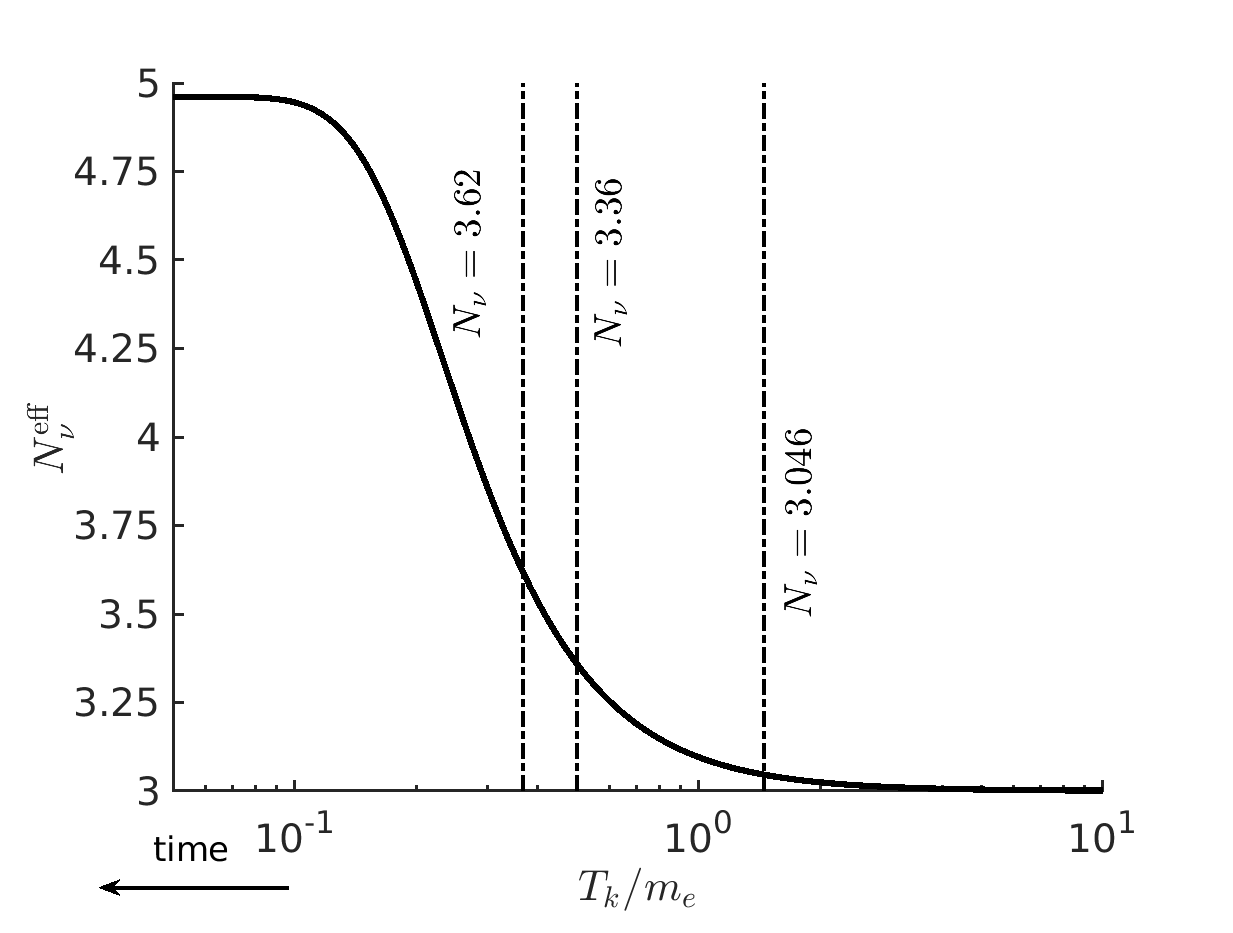
\includegraphics[height=5.4cm]{04-birrell/ModelIndStudy/Figures/N_eff.eps}}
\makebox[0.47\linewidth]%
{\hspace{4mm}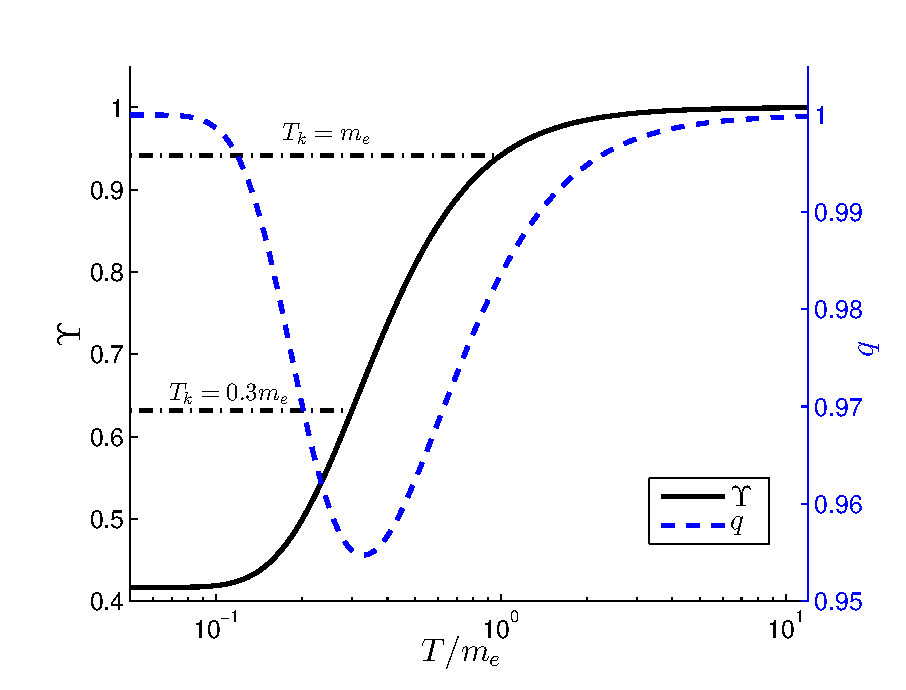
\includegraphics[height=5.5cm]{04-birrell/ModelIndStudy/Figures/Upsilon_q.eps}}
\caption{Dependence of  effective number of neutrinos (left) and neutrino fugacity (right) on the neutrino kinetic freeze-out temperature. We also show the evolution of the deceleration parameter through the freeze-out period (right).}
\end{minipage}
 \end{figure}
%%%%%%%%%%%%%%%%%%%%%%%%%%%%%%%%%%%%%%%


The conservation laws \req{eq_dynamics} and \req{const_entropy} then imply the following  relations.
\begin{enumerate}
\item Conservation of comoving neutrino number between chemical and kinetic freeze-out:
\begin{equation}\label{eq_1}
\frac{T_{ch}^3V(t_{ch})}{T_k^3V(t_k)}=\frac{2}{3\zeta(3)}\int_0^\infty \frac{u^2 du}{\Upsilon_\nu^{-1}(T_k)e^u+1}.
\end{equation}
\item Conservation of the entropy in $e^\pm$, $\gamma$, and neutrinos prior to neutrino freeze-out:
\begin{align}\label{eq_2}
&\left(\frac{7}{8}g_\nu+\frac{7}{8}g_{e^\pm} +g_\gamma \right)\frac{2\pi^2}{45} T_{ch}^3V(t_{ch})=\\
&\left(S_{\nu}(T_k)+S_{e^\pm}(T_k)+\frac{2\pi^2}{45}g_\gamma T_k^3\right)V(t_k)\,.\notag
\end{align}
\item Conservation of the entropy in $e^\pm$ and $\gamma$ between neutrino freeze-out and $e^\pm$ annihilation:
\begin{equation}\label{eq_3}
\frac{2 \pi^2}{45}g_\gamma T_{\gamma}^3 V(t)=\left(\frac{2\pi^2}{45}g_\gamma T_k^3+S_{e^\pm}(T_k)\right)V(t_k)\,, \,\,\, T_\gamma\ll \min\{m_e, T_k\}\,.
\end{equation}
\end{enumerate}
These relations allow one to solve for the fugacity, reheating ratio, and effective number of neutrinos in terms of the kinetic freeze-out temperature, irrespective of the details of the dynamics that leads to a particular freeze-out temperature. Specifically, combining \req{eq_1} and \req{eq_2}  one obtains
\begin{align}
   \frac{S_{\nu}(T_k)/T_k^3+S_{e^\pm}(T_k)/T_k^3+\frac{2\pi^2}{45}g_\gamma }{\left(\frac{7}{8}g_\nu+\frac{7}{8}g_{e^\pm} +g_\gamma \right)\frac{2\pi^2}{45} }=\frac{2}{3\zeta(3)}\int_0^\infty \frac{u^2 du}{\Upsilon_\nu^{-1}(T_k)e^u+1}.
\end{align}
This can be solved numerically to compute $\Upsilon_\nu(T_k)$. One can also use these relations to analytically derive the following expansion for the photon to neutrino temperature ratio after $e^\pm$ annihilation (see \cite{Birrell:2013_2}):
\begin{align}\label{Upsilon_ratio}
&\frac{T_\gamma}{T_\nu}=a\Upsilon^{b}\left(1+c\sigma^2+O(\sigma^3)\right),\\
\label{value_a}
&a=\left(1+\frac{7}{8}\frac{g_{e^\pm}}{g_\gamma}\right)^{1/3}=\left(\frac{11}{4}\right)^{1/3}\,,\,\,\,b\approx 0.367\,, \,\,\,c\approx -0.0209\,.\notag
\end{align}
An approximate power law fit was first obtained numerically in \cite{Birrell2013}. A relation between   the fugacity $\Upsilon=e^\sigma$ and the effective number of neutrinos \eqref{eq:N_eff_def} was also derived in \cite{Birrell:2013_2} using these methods:
\begin{equation}\label{N_nu_approx}
N^{\mathrm{eff}}_\nu=\frac{360}{7\pi^4}\frac{e^{-4b\sigma}}{(1+c\sigma^2)^4}\int_0^\infty \frac{u^3}{e^{u-\sigma}+1}du\left(1+O(\sigma^3)\right)\,.
\end{equation}
 In Figure \ref{fig:Tk_dependence} we plot that dependence of $N^{\mathrm{eff}}_\nu$ and $\Upsilon$  on $T_k$ that is implied by these calculations.  In particular, the fugacity evolves following the solid black curve in the right hand plot until it reaches the kinetic freeze-out temperature, at which point the neutrinos decouple and $\Upsilon$ remains constant thereafter, as shown in the dashed black curves for two sample values of $T_k$. Planck CMB results contain several fits~\cite{Planck} based on different data sets which suggest that $N^{\mathrm{eff}}_\nu$ is in the range $3.30\pm 0.27$ to $3.62\pm0.25$ ($68\%$ confidence level). A numerical computation based on the Boltzmann equation with two body scattering~\cite{Mangano2005} gives to $N_{\nu}^{\rm eff}=3.046$. These values are shown in the vertical lines in the left figure. The tension between the Planck results and theoretical reheating studies motivates our work.





%%%%%%%%%%%%%%%%%%%%%%%%%%%%%%%%%%%%%%%%%%%%%%%%%%%%%%%%%%%%%%%%%%%%
\subsection{Contribution to $N^{\text{eff}}_{\nu}$ of  Sub-eV  Mass Sterile Particles}\label{sec:Neff_QGP}

Moving beyond neutrinos, in this section we study the effect on $N_\nu^{\text{eff}}$ of non-SM light weakly coupled  particle species, referred to here as a sterile particles (SP),   generalizing the  sterile neutrino concept. We emphasize that such hypothetical SPs would behave as `dark radiation'~\cite{Steigman:2013yua} rather than cold dark matter.  This section is based on the work in \cite{Birrell:2014cja}.


{\bf ??? edit ???}
The possibility that Goldstone bosons  could be mistaken for fractional contribution to cosmic neutrinos was  identified in \cite{Weinberg:2013kea}.  Another viable candidate for SPs are sterile neutrinos. It has been shown that for three `new' right-handed neutrinos to fully account for the effective number of neutrinos, $N^{\text{eff}}_{\nu}$, the required freeze-out temperature required   is in the vicinity of the quark gluon plasma (QGP) phase transition~\cite{Anchordoqui:2011nh,Anchordoqui:2012qu}. Here we consider the QGP  phase transformation in the early Universe and evaluate quantitatively  the production and freeze-out of possible SPs in such a transition. If SPs are interpreted as Goldstone bosons, it would imply that in the deconfined phase there is  an additional hidden symmetry, weakly broken at hadronization.  For example, if this symmetry were to be part of the baryon conservation riddle, then we can expect that these Goldstone bosons will  couple to particles with baryon number, and possibly only in the domain where the vacuum is modified from its present day condition. 

The former paper proposed a concrete model of how this might be obtained from an expanded gauge group for QCD.  However,  the QGP equation of state (EoS) which were used are not consistent with recent numerical lattice-QCD results.   We use the  lattice-QCD derived QGP EoS from Ref.~\cite{Borsanyi:2013bia} to characterize the relation between $N^{\text{eff}}_{\nu}$ and the number of DoF that froze out at the time that the quark-gluon deconfined phase froze into hadrons near $T=150\MeV$, and  compute the coupling strength required to achieve freeze-out at the QGP transformation. 


The Einstein equations  imply a practically entropy conserving expansion of the Universe. Entropy conservation during periods when dimensional (mass) scales are irrelevant means that all temperatures scale inversely with the metric  scale factor $a(t)$. As temperature  passes through $m\simeq T$ thresholds, successively less massive particles annihilate and their entropy is shifted into the remaining effectively massless particles, causing the  $T\propto 1/a(t)$ scaling to break down. 


After an effectively massless particle species decouples, its temperature scales as $1/a(t)$ at all later times as a result of the free-streaming solution of the Einstein-Vlasov equation.  This leads to a temperature difference between the free streaming particles, and the photon background, which is the last to freeze-out. This reheating effect builds up during each  period  in which particle species disappear from the Universe inventory.

We denote by $S$ the conserved `comoving' entropy in a volume element $dV$, which scales with the factor $a(t)^3$. We define the effective number of entropy DoF, $g_*^S$, by
\begin{equation}
S=\frac{2\pi^2}{45}g^S_*T_\gamma^3 a^3.
\end{equation} 
For ideal Fermi and Bose gases
\begin{equation}
g_*^S=\!\!\!\!\sum_{i=\text{bosons}}\!\!\!\!g_i \left(\frac{T_i}{T_\gamma}\right)^3\!\!\!f_i^-+\frac{7}{8}\!\!\!\sum_{i=\text{fermions}}\!\!\!\! g_i \left(\frac{T_i}{T_\gamma}\right)^3\!\!\!f_i^+.
\end{equation}
The $g_i$ are degeneracies, $f_i^\pm$ are known functions, valued in $(0,1)$, that turn off the various species as the temperature drops below their mass-- compare to the analogous Eqs. (2.3) and (2.4) in Ref.\cite{Blennow:2012de}. 


%%%%%%%%%%%%%%%%%%%%%%%%%%%%%%%%%%%%%%%
\begin{figure}\label{fig:gs}
\centering
\begin{minipage}[b]{.49\textwidth}
\centerline{\hspace*{-0.10cm}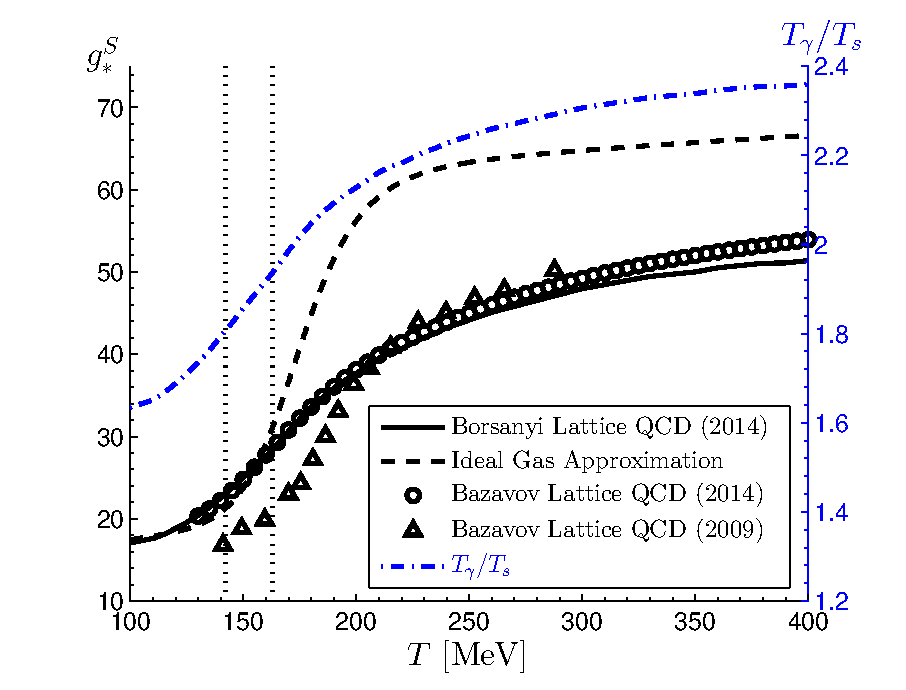
\includegraphics[height=6.4cm]{04-birrell/ModelIndStudy/Figures/gS_T_ratio.eps}}
\end{minipage}
\caption{\cccite{Birrell:2014cja}. Left axis: Effective number of entropy-DoF, including lattice QCD effects applying Ref.~\cite{Borsanyi:2013bia} (solid line) and  Ref.~\cite{HotQCD:2014kol} (circles), compared to the early Ref.\cite{Bazavov:2009zn} (triangles) results used by~\cite{Anchordoqui:2011nh}, and the ideal gas model of Ref.\cite{Coleman:2003hs} (dashed line) as function of temperature $T$. Right axis: Photon to SP temperature ratio, $T_\gamma/T_s$, as a function of SP decoupling temperature (dash-dotted (blue) line). The vertical dotted lines at $T=142$ and 163 MeV delimit the QGP transformation region.\label{fig:gS}}
 \end{figure}
%%%%%%%%%%%%%%%%%%%%%%%%%%%%%%%%%%%%%%%

Such a simple characterization does not hold in the vicinity of the QGP phase transformation where  quark-hadron degrees of freedom are strongly coupled  and the system must be studied using lattice QCD. This result is incorporated in the solid line in figure \ref{fig:gS} (left axis), where we have used a table of entropy density values through the QGP phase transition presented by Borsanyi et al.~\cite{Borsanyi:2013bia}, while circles show recent results from Bazavov et al.~\cite{HotQCD:2014kol}. This should be compared to the ideal gas approximation from~\cite{Coleman:2003hs} together with the fit in~\cite{Wantz:2009it} to interpolate though the QGP phase transition and older (year 2009) lattice data from Ref.\cite{Bazavov:2009zn} (triangles). The free gas approximation carries with it a maximum error of $10\%$ in the temperature range of the QGP phase transition  $T\simeq 150$\,MeV where quarks appear.  The error in the 2009 lattice data used in Ref.\cite{Anchordoqui:2011nh} is on the order of $25\%$.  This leads to a non-negligible difference in the relation between freeze-out temperature and $N^{\text{eff}}_{\nu}$.

%%%%%%%%%%%%%%%%%%%%%%%%%%%%%%%%%%%%%%%
\begin{figure}
\centering
\begin{minipage}[b]{.49\textwidth}
\centerline{\hspace*{0.4cm}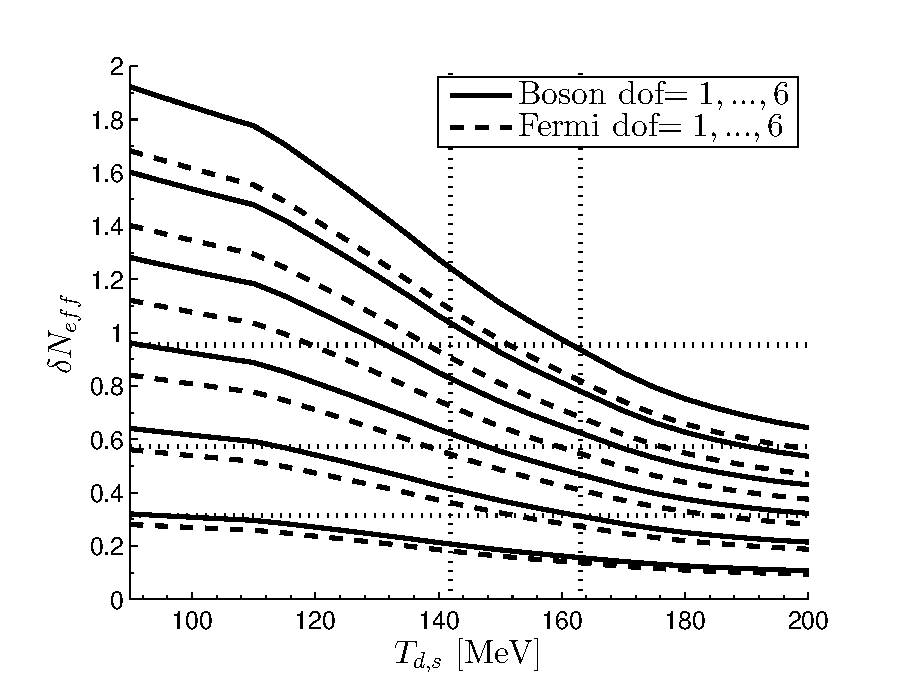
\includegraphics[height=6.8cm]{04-birrell/ModelIndStudy/Figures/Neff_Td_combined.eps}}
\end{minipage}
\caption{\cccite{Birrell:2014cja}. Solid lines: Increase in $\delta N_{\text{eff}}$ due to the effect of $1,\dots,6$ light sterile boson DoF ($g_s=1,\dots,6$, bottom to top curves) as a function of freeze-out temperature $T_{d,s}$. Dashed lines: Increase in $\delta N_{\text{eff}}$ due to the effect of $1,\dots,6$ light sterile fermion DoF ($g_s=7/8\times 1,\dots,7/8\times 6$, bottom to top curves) as a function of freeze-out temperature $T_{d,s}$. The horizontal dotted lines correspond to $\delta N_{\text{eff}}+0.046=0.36,0.62,1$. The vertical dotted lines show the reported range of QGP transformation temperatures $T_c=142-163\MeV$.\label{fig:Neff_Td_zoom}}
\end{figure}
%%%%%%%%%%%%%%%%%%%%%%%%%%%%%%%%%%%%


Once the SPs decouple from the  particle inventory at a photon temperature of $T_{d,s}$, a difference in their temperature from that of photons will build up during subsequent photon reheating periods, as discussed above. Conservation of entropy leads to a temperature ratio at $T_\gamma<T_{d,s}$, shown in the dot-dashed line in figure \ref{fig:gS} (right axis), of
\begin{equation}\label{T_ratio}
R_s\equiv T_{s}/T_{\gamma}=\left(\frac{g_*^S(T_\gamma)}{g_*^S(T_{d,s})}\right)^{1/3}.
\end{equation}


If $T_s$ and $T_\gamma$ are the light SP and photon temperatures, both after $e^\pm$ annihilation, and $g_s$ is the number of DoF of the SPs normalized to bosons (i.e. for fermions it includes an additional factor of $7/8$) then this gives
\begin{equation}\label{Neff1}
\delta N_{\text{eff}}\equiv N^{\text{eff}}_{\nu}-3.046=\frac{4g_s}{7}\left(\frac{T_s}{R_s T_{\gamma}}\right)^4
\end{equation}
where $3.046$ is the SM neutrino contribution. Using \req{T_ratio} we can rewrite $\delta N_{\text{eff}}$ as
\begin{equation}\label{delta_N}
\delta N_{\text{eff}}=\frac{4g_s}{7R_\nu^4}\left(\frac{g_*^S(T_{\gamma})}{g_*^S(T_{d,s})}\right)^{4/3}.
\end{equation}
where   $T_{d,s}$ is the decoupling temperature of the SP and $T_{\gamma}$ is any photon temperature $T_{\gamma}\ll m_e$. The SM particles remaining at $T_{\gamma}$ are  photons and SM neutrinos, the latter with temperature $R_\nu T_{\gamma}$, and so $g_*^S(T_{\gamma})=2+7/8\times 6\times 4/11$ and (see also Eq.(2.7) in~\cite{Blennow:2012de})
\begin{align}\label{delta_N2}
\delta N_{\text{eff}}\approx&g_s\left(\frac{7.06}{g_*^S(T_{d,s})}\right)^{4/3}.
\end{align}

Figure \ref{fig:Neff_Td_zoom} shows $\delta N_{\text{eff}}$ as a function of $T_{d,s}$ for $1,\dots,6$ boson (solid lines) and fermion (dashed lines) DoF. For a low decoupling temperature $T_{d,s}<100$\,MeV  a single bose or fermi SP  can help alleviate the tension in $N^{\text{eff}}_{\nu}$. Within QGP hadronization interval $T_c=142-163\MeV$ (marked by vertical lines) we see that three bose degrees of freedom or four fermi degrees of freedom are the most likely cases to resolve the tension. 

It is also clear from  figure \ref{fig:Neff_Td_zoom} that the rapid growth of the number of degrees of freedom in the QGP phase implies that earlier decoupling temperatures lead to a rapid increase in the required number of SPs. While one cannot exclude the possible presence of 20--30 new dark light particles, it seems to us unlikely that there are that many undiscovered weakly broken symmetries producing light Goldstone, or/and sterile neutrino-like particles. We believe that figure \ref{fig:Neff_Td_zoom}  pinpoints the QGP  temperature range and below as the primary domain of interest for the freeze-out of such hypothetical degrees of freedom, should these be responsible for the modification $\delta N_{\text{eff}}$.





